\section{System Implementation} 
As can be deduced from the above overview, the system is quite complex,
this means that there has been some challenges when building the system.

Initially the concept was to have pure bluetooth communication between the 3 main components,
but due to unexpected challenges a fourth element was introduced to handle communication between android and the weka system. 
However this also means that the system is not limited by the short range of the bluetooth receiver.
The communication flow we ended up with is shown in figure \ref{fig:sys}.

\subsection{Gesture Recognition}
The gesture recognition is done in multiple steps, since the system has been designed not to preprocess the data on the MTD.
The first step is preprocessing and the second is classifying or evaluating.

\subsubsection{Preprocessing}
Once the acceleration and rotation data is sent from the device to the computer,
 the values are smoothed with an average of the 20 previous values in order to avoid and reduce the effect of noise on the sensors.
 This phase is called preprocessing of the data. 
 This allowed us to have more precise information, as can be deducted from the images  \ref{fig:figure2} and \ref{fig:figure3}

\begin{figure}[h]
\centering
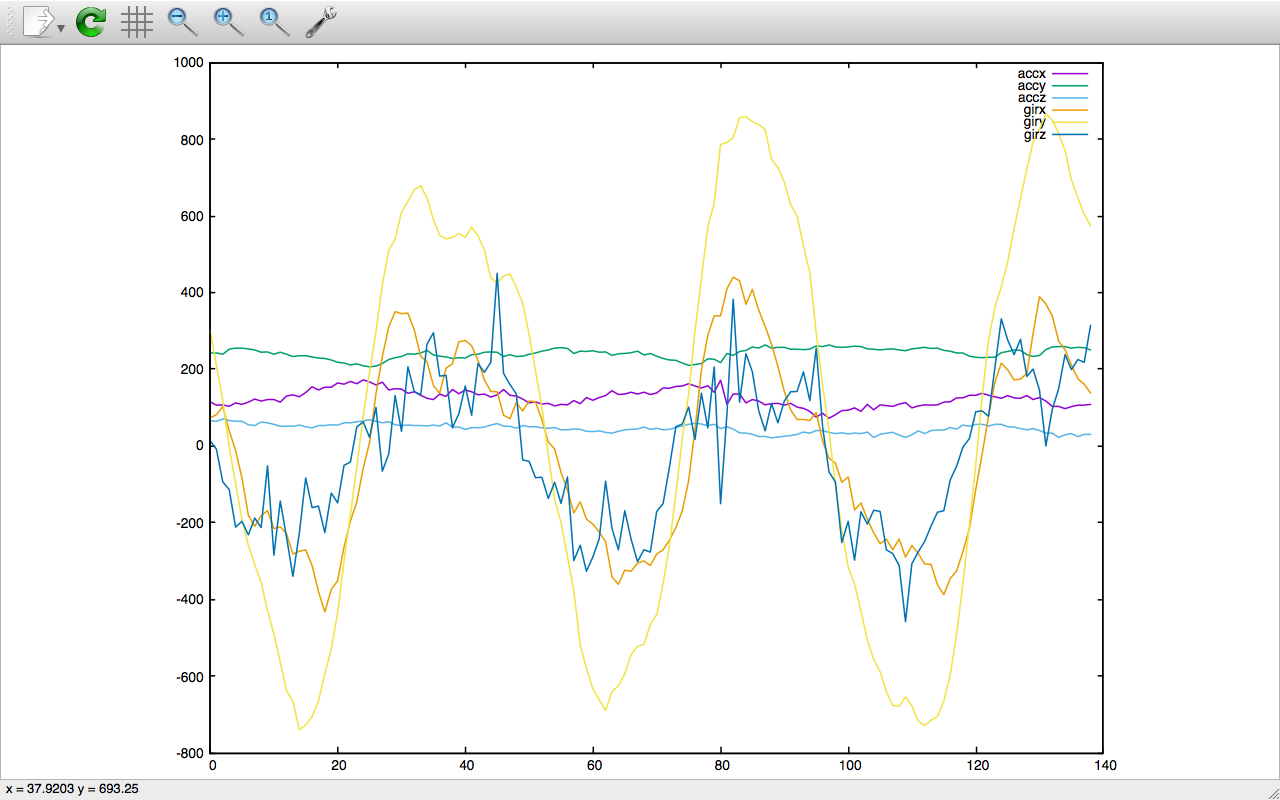
\includegraphics[width=1\columnwidth]{img/raw}
\caption{Data from the device before preprocessing.}
\label{fig:figure2}
\end{figure}

\begin{figure}[h]
\centering
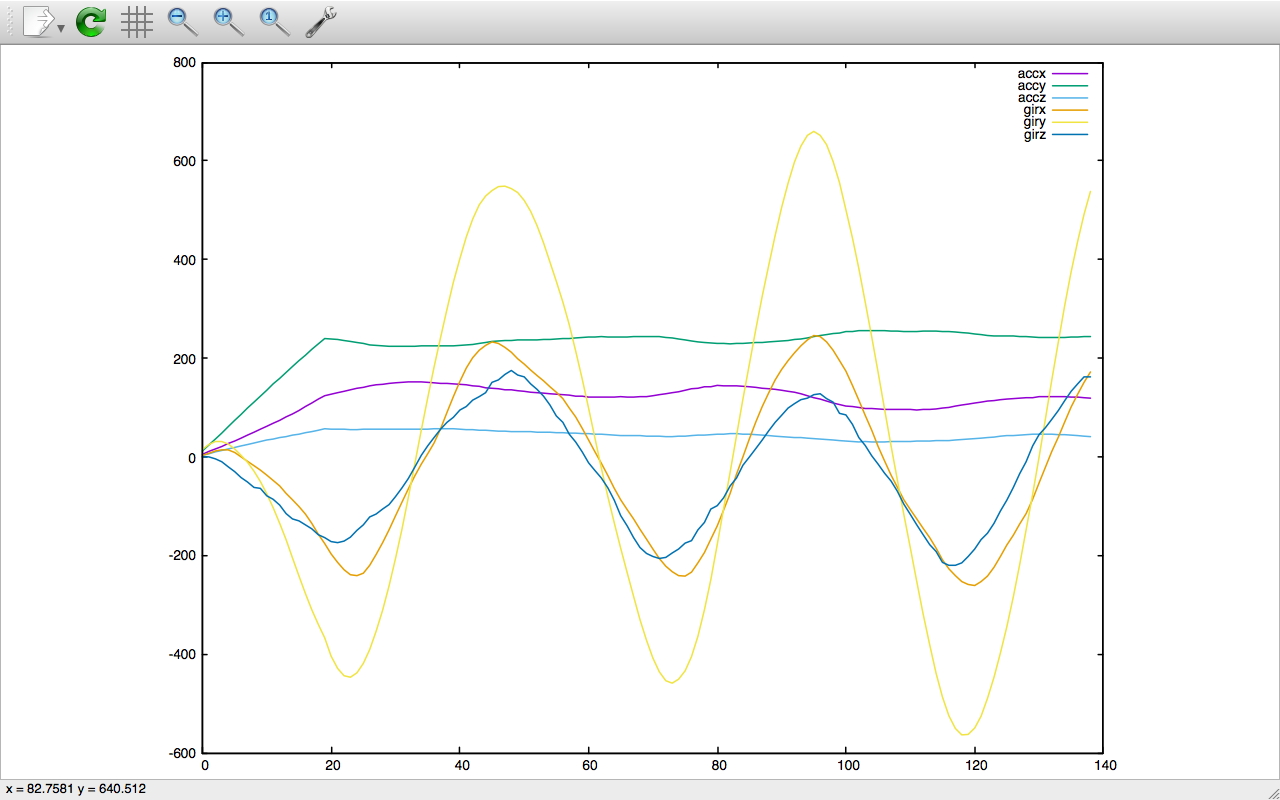
\includegraphics[width=1\columnwidth]{img/20}
\caption{Data from the device after preprocessing.}
\label{fig:figure3}
\end{figure}

\subsubsection{Evaluation}
For the actual processing and gesture recognition, we use a sliding window approach on the time series data we receive.
The window is of size 50, hence it will evaluate a sequence of 50 movement instances in a sequence,
every instance consisting of 6 values.

The window is able to capture a period of time of about 2 seconds, as the sampling rate of the device is about 25 Hz.

We organized known gestures in a very large training set, each individual gesture stored as a list of 50 * 6 values plus an identifier, in a way that every gesture will be compatible with the sliding window. 

The training data set in the final version of the project reached more than 500 entries in total.
This was achieved by automatically storing multiple entries for each single gesture.

Every gesture was intentionally registered on a larger interval than the one used for the sliding evaluation window.
In this way, being every entry of the training set of size 50,  each gesture was entered multiple times, one for each of its subsets of 50 subsequent instances.
The number of entries for the same gesture is usually not fixed and in general it depends on the gesture itself, however it usually varies between 1 and 30.\\
This process is depicted in figure \ref{fig:training}

\begin{figure}[!h]
\centering
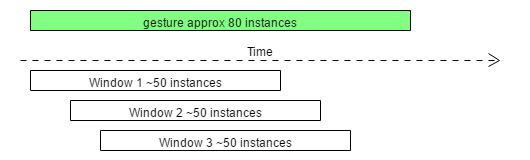
\includegraphics[width=1\columnwidth]{img/gesture_window_example}
\caption{Storing a bigger gesture in the training data set.}
\label{fig:training}
\end{figure}

The evaluation of the gesture is performed every 10 * 6 new values received,
 and being that every gesture is stored in the different phases of its conduct,
  the likelihood of evaluating gestures that are in unknown phases and therefore not recognized is lower.

We use Weka 3.6 to evaluate newly received data using a BayesNet classifier and comparing it to the training set. 
This resulted as one of the most accurate classifiers for our model, giving up to 100\% accuracy in the testing phase of the project. A comparison with other classifiers is shown in figure \ref{fig:wekaclass}.

\begin{figure}[h]
\begin{center}
\begin{tabular}{ l  c r }
Classifier & Precision & Time(s)\\ [0.5ex]
\hline \hline
BayesNet & 100 \%  & 0.06\\ 
IBk & 100 \% & 0.1 \\
LWL & 77.3\%  & 1.86\\
REPTree & 95.5\%  & 0.03 \\ [1ex]
\end{tabular}
\end{center}
\caption{Test table for classifiers}
\label{fig:wekaclass}
\end{figure}

\begin{figure}[!h]
\centering
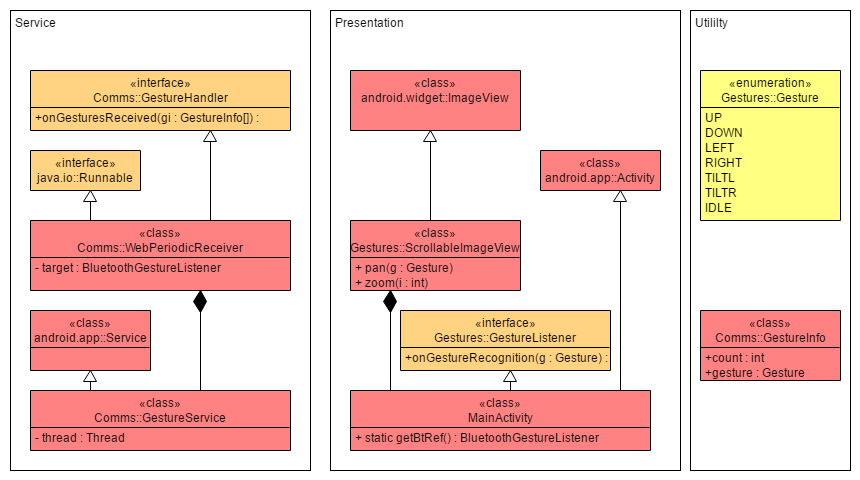
\includegraphics[width=1\columnwidth]{img/android_class_diagram}
\caption{Android Application Class diagram.}
\label{fig:and_class}
\end{figure}

\subsection{Webservice}
The communication between the android presenter app and the gesture recognition system is done using a simple webservice.
The webservice uses a queue and is therefore prone to both starvation and overflow
(in the sense that commands queue up to such a level that there will be a significant delay when handling them).

The way we handle these potential issues is quite different.
The starvation issues are handled on the android device with a simple null or 0 elements check on the web service results.
The overflow is handled by being able to discard all the queued elements using a DELETE request sent to the service.

\subsection{Android Image Presenter}
The android application has been designed to handle communication over a webservice in the background, 
while the presentation layer is done such that it is easily exchangeable due to an interface as seen on figure \ref{fig:and_class}.

The flow of information is quite simple, when the GestureService has a non-empty result from the webservice,
it propagates this information to the GestureHandler, which has knowledge about any GestureListener instance.

The Mainactivity.class implements the GestureListener.
A custom ImageView has been designed to expose functions needed such as zoom and pan, which are manipulated via the aforementioned listener.
